\documentclass[11pt]{mimosis}
\synctex=1

% \PassOptionsToClass{14pt}{scrbook}
\usepackage{metalogo}

\usepackage{textcomp}
\usepackage{gensymb}

\usepackage[pass]{geometry}

%%%%%%%%%%%%%%%%%%%%%%%%%%%%%%%%%%%%%%%%%%%%%%%%%%%%%%%%%%%%%%%%%%%%%%%%
% Some of my favorite personal adjustments
%%%%%%%%%%%%%%%%%%%%%%%%%%%%%%%%%%%%%%%%%%%%%%%%%%%%%%%%%%%%%%%%%%%%%%%%
%
% These are the adjustments that I consider necessary for typesetting
% a nice thesis. However, they are *not* included in the template, as
% I do not want to force you to use them.

% This ensures that I am able to typeset bold font in table while still aligning the numbers
% correctly.
\usepackage{etoolbox}

\usepackage[binary-units=true]{siunitx}
\DeclareSIUnit\px{px}

\sisetup{%
  detect-all           = true,
  detect-family        = true,
  detect-mode          = true,
  detect-shape         = true,
  detect-weight        = true,
  detect-inline-weight = math,
}

%%%%%%%%%%%%%%%%%%%%%%%%%%%%%%%%%%%%%%%%%%%%%%%%%%%%%%%%%%%%%%%%%%%%%%%%
% Hyperlinks & bookmarks
%%%%%%%%%%%%%%%%%%%%%%%%%%%%%%%%%%%%%%%%%%%%%%%%%%%%%%%%%%%%%%%%%%%%%%%%

\usepackage[%
  colorlinks = true,
  citecolor  = BrickRed,
  linkcolor  = BrickRed,
  urlcolor   = BrickRed,
  % pdftex,
  pdfauthor={Jan Straub},
  pdftitle={Reflections on the correlation between the tendency to procrastinate and the likelihood to be awarded a doctoral degree},
  % pdfsubject={The Subject},
  % pdfkeywords={Some Keywords},
  % pdfproducer={Latex with hyperref, or other system},
  % pdfcreator={pdflatex, or other tool}
  ]{hyperref}

\usepackage{bookmark}


%%%%%%%%%%%%%%%%%%%%%%%%%%%%%%%%%%%%%%%%%%%%%%%%%%%%%%%%%%%%%%%%%%%%%%%%
% Bibliography
%%%%%%%%%%%%%%%%%%%%%%%%%%%%%%%%%%%%%%%%%%%%%%%%%%%%%%%%%%%%%%%%%%%%%%%%
%
% I like the bibliography to be extremely plain, showing only a numeric
% identifier and citing everything in simple brackets. The first names,
% if present, will be initialized. DOIs and URLs will be preserved.

\usepackage[%
  autocite      = plain,
  backend       = biber,
  doi           = false,
  url           = true,
  giveninits    = true,
  hyperref      = true,
  maxbibnames   = 99,
  maxcitenames  = 99,
  sortcites     = true,
  style         = alphabetic,
  citestyle     = alphabetic,
  maxalphanames = 4,           % max number of authors before it becomes [First+12]
  backref       = true,
  ]{biblatex}


%%%%%%%%%%%%%%%%%%%%%%%%%%%%%%%%%%%%%%%%%%%%%%%%%%%%%%%%%%%%%%%%%%%%%%%%
% Some adjustments to make the bibliography more clean
%%%%%%%%%%%%%%%%%%%%%%%%%%%%%%%%%%%%%%%%%%%%%%%%%%%%%%%%%%%%%%%%%%%%%%%%
%
% The subsequent commands do the following:
%  - Removing the month field from the bibliography
%  - Fixing the Oxford commma
%  - Suppress the "in" for journal articles
%  - Remove the parentheses of the year in an article
%  - Delimit volume and issue of an article by a colon ":" instead of
%    a dot ""
%  - Use commas to separate the location of publishers from their name
%  - Remove the abbreviation for technical reports
%  - Display the label of bibliographic entries without brackets in the
%    bibliography
%  - Ensure that DOIs are followed by a non-breakable space
%  - Use hair spaces between initials of authors
%  - Make the font size of citations smaller
%  - Fixing ordinal numbers (1st, 2nd, 3rd, and so) on by using
%    superscripts

% Remove the month field from the bibliography. It does not serve a good
% purpose, I guess. And often, it cannot be used because the journals
% have some crazy issue policies.
\AtEveryBibitem{\clearfield{month}}
\AtEveryCitekey{\clearfield{month}}

% Fixing the Oxford comma. Not sure whether this is the proper solution.
% More information is available under [1] and [2].
%
% [1] http://tex.stackexchange.com/questions/97712/biblatex-apa-style-is-missing-a-comma-in-the-references-why
% [2] http://tex.stackexchange.com/questions/44048/use-et-al-in-biblatex-custom-style
%
\AtBeginBibliography{%
  \renewcommand*{\finalnamedelim}{%
    \ifthenelse{\value{listcount} > 2}{%
      \addcomma
      \addspace
      \bibstring{and}%
    }{%
      \addspace
      \bibstring{and}%
    }
  }
}

% Suppress "in" for journal articles. This is unnecessary in my opinion
% because the journal title is typeset in italics anyway.
\renewbibmacro{in:}{%
  \ifentrytype{article}
  {%
  }%
  % else
  {%
    \printtext{\bibstring{in}\intitlepunct}%
  }%
}

% Remove the parentheses for the year in an article. This removes a lot
% of undesired parentheses in the bibliography, thereby improving the
% readability. Moreover, it makes the look of the bibliography more
% consistent.
\renewbibmacro*{issue+date}{%
  \setunit{\addcomma\space}
    \iffieldundef{issue}
      {\usebibmacro{date}}
      {\printfield{issue}%
       \setunit*{\addspace}%
       \usebibmacro{date}}%
  \newunit}

% Delimit the volume and the number of an article by a colon instead of
% by a dot, which I consider to be more readable.
\renewbibmacro*{volume+number+eid}{%
  \printfield{volume}%
  \setunit*{\addcolon}%
  \printfield{number}%
  \setunit{\addcomma\space}%
  \printfield{eid}%
}

% Do not use a colon for the publisher location. Instead, connect
% publisher, location, and date via commas.
\renewbibmacro*{publisher+location+date}{%
  \printlist{publisher}%
  \setunit*{\addcomma\space}%
  \printlist{location}%
  \setunit*{\addcomma\space}%
  \usebibmacro{date}%
  \newunit%
}

% Ditto for other entry types.
\renewbibmacro*{organization+location+date}{%
  \printlist{location}%
  \setunit*{\addcomma\space}%
  \printlist{organization}%
  \setunit*{\addcomma\space}%
  \usebibmacro{date}%
  \newunit%
}

% Do not abbreviate "technical report".
\DefineBibliographyStrings{english}{%
  techreport = {technical report},
}

% Display the label of a bibliographic entry in bare style, without any
% brackets. I like this more than the default.
%
% Note that this is *really* the proper and official way of doing this.
\DeclareFieldFormat{labelnumberwidth}{#1\adddot}

% Ensure that DOIs are followed by a non-breakable space.
\DeclareFieldFormat{doi}{%
  \mkbibacro{DOI}\addcolon\addnbspace
    \ifhyperref
      {\href{http://dx.doi.org/#1}{\nolinkurl{#1}}}
      %
      {\nolinkurl{#1}}
}

% Use proper hair spaces between initials as suggested by Bringhurst and
% others.
\renewcommand*\bibinitdelim {\addnbthinspace}
\renewcommand*\bibnamedelima{\addnbthinspace}
\renewcommand*\bibnamedelimb{\addnbthinspace}
\renewcommand*\bibnamedelimi{\addnbthinspace}

% Make the font size of citations smaller. Depending on your selected
% font, you might not need this.
\renewcommand*{\citesetup}{%
  \biburlsetup
  \small
}

% \DeclareLanguageMapping{british}{bibliography-correct-ordinals}
% \DeclareLanguageMapping{english}{bibliography-correct-ordinals}
\bibliography{Thesis}

%%%%%%%%%%%%%%%%%%%%%%%%%%%%%%%%%%%%%%%%%%%%%%%%%%%%%%%%%%%%%%%%%%%%%%%%
% Fonts
%%%%%%%%%%%%%%%%%%%%%%%%%%%%%%%%%%%%%%%%%%%%%%%%%%%%%%%%%%%%%%%%%%%%%%%%

\ifxetexorluatex
  %\setmainfont{Minion Pro}
  \usepackage{microtype}
\else
  %\usepackage[osf,lining]{ebgaramond}  
  \usepackage[scale=0.7]{sourcecodepro}  
\fi






\usepackage{mathpazo}
\usepackage{lettrine}

\usepackage{makeidx}
\makeindex



% \newacronym[description={Principal component analysis}]{PCA}{PCA}{principal component analysis}
% \newacronym                                            {SNF}{SNF}{Smith normal form}
% \newacronym[description={Topological data analysis}]   {TDA}{TDA}{topological data analysis}

% \makeindex
% \makeglossaries

%%%%%%%%%%%%%%%%%%%%%%%%%%%%%%%%%%%%%%%%%%%%%%%%%%%%%%%%%%%%%%%%%%%%%%%%
% Incipit
%%%%%%%%%%%%%%%%%%%%%%%%%%%%%%%%%%%%%%%%%%%%%%%%%%%%%%%%%%%%%%%%%%%%%%%%
 
\usepackage{mathtools}
\usepackage{amssymb}
\usepackage{siunitx}

\usepackage{blindtext}

% Corrects \autoref{}: chapter -> Chapter, section -> Section, subsection -> Section
\addto\extrasenglish{%
  \renewcommand{\chapterautorefname}{Chapter}%
  \renewcommand{\sectionautorefname}{Section}%
  \renewcommand{\subsectionautorefname}{Section}%
}

\begin{document}

\frontmatter
  %!TEX root = ../Thesis.tex

\begin{titlepage}
  \centering % Center all text
  \vspace*{\baselineskip} % White space at the top of the page

  %\rule{\textwidth}{1.6pt}\vspace*{-\baselineskip}\vspace*{2pt} % Thick horizontal line
  %\rule{\textwidth}{0.4pt}\\[1.0\baselineskip] % Thin horizontal line

  {\huge Visualization of Heat Waves}\\[0.2\baselineskip] % Title

  %\rule{\textwidth}{0.4pt}\vspace*{-\baselineskip}\vspace{3.2pt} % Thin horizontal line
  %\rule{\textwidth}{1.6pt}\\ % Thick horizontal line

  \vspace*{\baselineskip}

  {\Large Bachelor's Thesis\\[\baselineskip]} % Tagline(s) or further description
  \vspace*{\baselineskip}

  {\LARGE Jan Michael Straub\\[\baselineskip]} % Editor list  

  \vspace*{\baselineskip} % Whitespace between location/year and editors

  Supervisor\\
  {\large  Prof.\,Dr.\,Filip Sadlo\\[\baselineskip]} % Editor list

  \vfil

  Heidelberg,  \today \par % Location and year

  \vspace*{\baselineskip}

  {\itshape Faculty of Mathematics and Computer Science\par} % Editor affiliation
  {\itshape Heidelberg University\par} % Editor affiliation
\end{titlepage}

\cleardoublepage

  % %!TEX root = ../Thesis.tex

\selectlanguage{english}

\begin{titlepage}
  \begin{center}
    \textsc{\huge Dissertation}
                \vskip 1cm
                \begin{large}
                  submitted to the\\[0.50cm]
                  \begin{Large}
                    \textsc{Combined Faculty for the\\Natural Sciences and Mathematics}\\[0.50cm]
                  \end{Large}
                  of\\[0.50cm]
                  \begin{Large}
                    \textsc{Heidelberg University, Germany}\\[0.50cm]
                  \end{Large}
                  for the degree of \\[0.5cm] 
                  Doctor of Natural Sciences
                \end{large}
    %
    \vfill
    %
    \begin{large}
                  put forward by\\[0.5cm]
                  \begin{LARGE}
                    \textbf{Guybrush Threepwood}, M.Sc.
                  \end{LARGE}\\[0.5cm]
                  born in Ankh-Morpork, Discworld
    \end{large}
    %
    \vskip 2cm
    %
    \begin{small}
      Heidelberg\\
      Marchtember 2033
    \end{small}
  \end{center}
\end{titlepage}

\selectlanguage{english}

\begin{titlepage}
  %
  \phantom{}
  \vfill 
  %
  \begin{center}
    \begin{singlespace*}
      \begin{Huge}
          Reflections on the correlation between the tendency to procrastinate and the likelihood to be awarded a doctoral degree\par
      \end{Huge}
      %
      \vskip 0.25cm
      \emph{by}
      \vskip 0.25cm
      %
      \textsc{Guybrush Threepwood}\par
    \end{singlespace*}
  \end{center}
  %
  \vfill
  %
  \begin{singlespace*}
    Advisor:            Prof.\,Dr.\,Filip Sadlo \\[.5cm]
    Oral examination: \rule{4cm}{0.15mm}
  \end{singlespace*}
\end{titlepage}

\newpage
\null
\thispagestyle{empty}
\newpage
  % for PhD thesis
  \pagestyle{empty}
  %!TEX root = ../Thesis.tex

\section*{Declaration of Authorship}

I hereby declare that the thesis submitted is my own unaided work. All direct or indirect sources used are acknowledged as references. The principles and recommendations \enquote{Verantwortung in der Wissenschaft} of Heidelberg University have been followed.
\vspace{5cm}\\
\noindent\rule[0.5ex]{8em}{0.5pt} \hfill \rule[0.5ex]{10em}{0.5pt}\\
\noindent Jan Straub \hfill Heidelberg, date and signature  % remove for PhD thesis
  %!TEX root = ../Thesis.tex
%%%%%%%%%%%%%%%%%%%%%%%%%%%%%%%%%%%%%%%%%%%%%%%%%%%%%%%%%%%%%%%%%%%%%%%%
\begin{center}
  \textsc{Abstract}
\end{center}
\noindent

In this thesis, we presented a novel edge bundling technique based on a Physarium approximation of a Steiner tree. Here we use the Steiner tree as a routing structure for graph paths. The resulting drawings consist of densely bundled graphs that reduce node-edge overlaps and make it easier to get an overview of the graph data.

For the Physarium calculation, we utilize the network Poisson equation to simulate a liquid flow inside the graph network, which enables us to cut nodes and edges, if the conductivity in an edge gets too low. Cutting edges shrinks the network until just a Steiner tree is left. To optimize the process, we multithreaded the calculation and found optimal iteration bounds that still deliver a satisfactory approximation result.
To visualize the initial network paths, we route them via the Steiner tree and visualize them by utilizing B\'{e}zier curves.

The outcomes enhance readability and make spotting areas of interest more straightforward. We further evaluate our algorithm by calculating the quality metrics: ink reduction, distortion, and ambiguity. We compare the results to two edge bundling approaches to classify our technique and comprehend its usefulness. We additionally discuss the constraints of our method and propose further improvements to circumvent these limitations.
%%%%%%%%%%%%%%%%%%%%%%%%%%%%%%%%%%%%%%%%%%%%%%%%%%%%%%%%%%%%%%%%%%%%%%%%

\cleardoublepage

  %!TEX root = ../Thesis.tex

\begin{center}
  \textsc{Zusammenfassung}
\end{center}
%
\selectlanguage{ngerman}
\noindent 

Diese Arbeit stellt einen neuen edge bundling Ansatz vor, welcher die Approximierung von Steinerbäumen mittels einer Physariumapproximierung durchführt. Der Steinerbaum wird dann als Struktur für das Routing von den ursprünglichen Graph Pfaden benutzt. Die resultierenden Darstellungen bestehen aus dichten Graphen, deren Knoten-Kanten Überschneidungen reduziert wurden und es dadurch einfacher ist, sich einen Überblick über die Daten zu verschaffen.

Für die Physariumapproximierung nutzten wir die Netzwerk-Poisson-Gleichung, um einen Fluss von Flüssigkeit im Graph zu simulieren. Sobald die Leitfähigkeit einer Kante zu gering wird, wird diese gelöscht. Dies führt dazu, dass der Graph sich immer weiter zusammenzieht, bis am Ende ein Steinerbaum übrigbleibt. Um den Prozess zu optimieren, haben wir für die Berechnungen Multithreading benutzt und die optimalen Iterationsgrenzen gefunden, welche trotzdem noch eine zufriedenstellende Approximation erreichen.
Um die ursprünglichen Graph Pfade darzustellen, suchen wir den besten Weg durch den Steinerbaum und stellen diesen dann mit Hilfe einer Bezierkurve dar.

Für die Evaluierung unserer Methode nutzen wir die Qualitätsmerkmale: Tintenreduzierung, Verzerrung und Mehrdeutigkeit. Die Ergebnisse vergleichen wir mit zwei anderen Ansätzen, um unseren Ansatz einordnen zu können und seinen Nutzen zu verstehen. Außerdem besprechen wir die Einschränkungen unserer Idee und schlagen möglichen Verbesserungen vor.

\selectlanguage{english}
\cleardoublepage

  \tableofcontents

\mainmatter
  \pagestyle{scrheadings}

  %!TEX root = ../Thesis.tex

%%%%%%%%%%%%%%%%%%%%%%%%%%%%%%%%%%%%%%%%%%%%%%%%%%%%%%%%%%%%%%%%%%%%%%%%
\chapter{Introduction}
%%%%%%%%%%%%%%%%%%%%%%%%%%%%%%%%%%%%%%%%%%%%%%%%%%%%%%%%%%%%%%%%%%%%%%%%

\begin{figure}[t]
  \centering
  
\includegraphics[width=0.5\linewidth]{figures/dummy}
  \caption{Do not state the obvious. Do not state the obvious. Do not state the obvious. Do not state the obvious. Do not state the obvious. Do not state the obvio.}
\end{figure}

But I must explain to you how all this mistaken \hyperref[sec:index]{idea}\index{idea} of denouncing pleasure and praising pain was born and I will give you a complete account of the system, and expound the actual teachings of the great explorer of the truth, the master-builder of human happiness. No one rejects, dislikes, or avoids pleasure itself, because it is pleasure, but because those who do not know how to pursue pleasure rationally encounter consequences that are extremely painful. Nor again is there anyone who loves or pursues or desires to obtain pain of itself, because it is pain, but because occasionally circumstances occur in which toil and pain can procure him some great pleasure. 

To take a trivial example, which of us ever undertakes laborious physical exercise, except to obtain some advantage from it? But who has any right to find fault with a man who chooses to enjoy a pleasure that has no annoying consequences, or one who avoids a pain that produces no resultant pleasure? On the other hand, we denounce with righteous indignation and dislike men who are so beguiled and demoralized by the charms of pleasure of the moment, so blinded by desire, that they cannot foresee the pain and trouble that are bound to ensue; and equal blame belongs to those who fail in their duty through weakness of will, which is the same as saying through shrinking from toil and pain. These cases are perfectly simple and easy to distinguish. In a free hour, when our power of choice is untrammelled and when nothing prevents our being able to do what we like best, every pleasure is to be welcomed and every pain avoided. But in certain circumstances and owing to the claims of duty or the obligations of business it will frequently occur that pleasures have to be repudiated and annoyances accepted. The wise man therefore always holds in these matters to this principle of selection: he rejects pleasures to secure other greater pleasures, or else he endures pains to avoid worse pains. 

But I must explain to you how all this mistaken \hyperref[sec:index]{idea}\index{idea} of denouncing pleasure and praising pain was born and I will give you a complete account of the system, and expound the actual teachings of the great explorer of the truth, the master-builder of human happiness. No one rejects, dislikes, or avoids pleasure itself, because it is pleasure, but because those who do not know how to pursue pleasure rationally encounter consequences that are extremely painful. Nor again is there anyone who loves or pursues or desires to obtain pain of itself, because it is pain, but because occasionally circumstances occur in which toil and pain can procure him some great pleasure. To take a trivial example, which of us ever undertakes laborious physical exercise, except to obtain some advantage from it? But who has any right to find fault with a man who chooses to enjoy a pleasure that has no annoying consequences, or one who avoids a pain that produces no resultant pleasure? On the other hand, we denounce with righteous indignation and dislike men who are so beguiled and demoralized by the charms of pleasure of the moment, so blinded by desire, that they cannot foresee the pain and trouble that are bound to ensue; and equal blame belongs to those who fail in their duty through weakness of will, which is the same as saying through shrinking from toil and pain. These cases are perfectly simple and easy to distinguish. In a free hour, when our power of choice is untrammelled and when nothing prevents our being able to do what we like best, every pleasure is to be welcomed and every pain avoided. But in certain circumstances and owing to the claims of duty or the obligations of business it will frequently occur that pleasures have to be repudiated and annoyances accepted. The wise man therefore always holds in these matters to this principle of selection: he rejects pleasures to secure other greater pleasures, or else he endures pains to avoid worse pains. But I must explain to you how all this mistaken \hyperref[sec:index]{idea}\index{idea} of denouncing pleasure and praising pain was born and I will give you a complete account of the system, and expound the actual teachings of the great explorer of the truth, the master-builder of human happiness. No one rejects, dislikes, or avoids pleasure itself, because it is pleasure, but because those who do not know how to pursue pleasure rationally encounter consequences that are extremely painful.

Nor again is there anyone who loves or pursues or desires to obtain pain of itself, because it is pain, but because occasionally circumstances occur in which toil and pain can procure him some great pleasure. To take a trivial example, which of us ever undertakes laborious physical exercise, except to obtain some advantage from it? But who has any right to find fault with a man who chooses to enjoy a pleasure that has no annoying consequences, or one who avoids a pain that produces no resultant pleasure? On the other hand, we denounce with righteous indignation and dislike men who are so beguiled and demoralized by the charms of pleasure of the moment, so blinded by desire, that they cannot foresee the pain and trouble that are bound to ensue; and equal blame belongs to those who fail in their duty through weakness of will, which is the same as saying through shrinking from toil and pain. These cases are perfectly simple and easy to distinguish. 

In a free hour, when our power of choice is untrammelled and when nothing prevents our being able to do what we like best, every pleasure is to be welcomed and every pain avoided. But in certain circumstances and owing to the claims of duty or the obligations of business it will frequently occur that pleasures have to be repudiated and annoyances accepted. The wise man therefore always holds in these matters to this principle of selection: he rejects pleasures to secure other greater pleasures, or else he endures pains to avoid worse pains. But I must explain to you how all this mistaken \hyperref[sec:index]{idea}\index{idea} of denouncing pleasure and praising pain was born and I will give you a complete account of the system, and expound the actual teachings of the great explorer of the truth, the master-builder of human happiness. No one rejects, dislikes, or avoids pleasure itself, because it is pleasure, but because those who do not know how to pursue pleasure rationally encounter consequences that are extremely painful. Nor again is there anyone who loves or pursues or desires to obtain pain of itself, because it is pain, but because occasionally circumstances occur in which toil and pain can procure him some great pleasure. To take a trivial example, which of us ever undertakes laborious physical exercise, except to obtain some advantage from it? But who has any right to find fault with a man who chooses to enjoy a pleasure that has no annoying consequences, or one who avoids a pain that produces no resultant pleasure? On the other hand, we denounce with righteous indignation and dislike men who are so beguiled and demoralized by the charms of pleasure of the moment, so blinded by desire, that they cannot foresee the pain and trouble that are bound to ensue; and equal blame belongs to those who fail in their duty through weakness of will, which is the same as saying through shrinking from toil and pain. 
  %!TEX root = ../Thesis.tex

%%%%%%%%%%%%%%%%%%%%%%%%%%%%%%%%%%%%%%%%%%%%%%%%%%%%%%%%%%%%%%%%%%%%%%%%
\chapter{Related Work}
\label{sec:relatedWork}
%%%%%%%%%%%%%%%%%%%%%%%%%%%%%%%%%%%%%%%%%%%%%%%%%%%%%%%%%%%%%%%%%%%%%%%%

\Blindtext[12] Do not forget to use references~\cite{Hanser2019energy} like done here~\cite{Hofmann2019dependentVectors} to enable the bibliography~\cite{Jung2017tumble, Sagrista2019GaiaSky, Sdeo2018fullerene, Zheng2019equivalence}.
  %!TEX root = ../Thesis.tex

%%%%%%%%%%%%%%%%%%%%%%%%%%%%%%%%%%%%%%%%%%%%%%%%%%%%%%%%%%%%%%%%%%%%%%%%
\chapter{Results}
\label{chap:Results}

The result of this thesis is a novel edge bundling algorithm that uses a Physarium Steiner tree calculation to build a structure that can then use to bundle the paths. As mentioned in \autoref{sec:testing}, we generated the graphs that we then compared to the Edge-Path bundling approach by Wallinger et al. \cite{wallinger_edge-path_2022}, and the Winding Roads method by Lambert et al. \cite{lambert_winding_2010}, as these have made their algorithms readily available, we already have a good understanding of how they work, and they are representative of a method with an underlying structure and one without one.

%%%%%%%%%%%%%%%%%%%%%%%%%%%%%%%%%%%%%%%%%%%%%%%%%%%%%%%%%%%%%%%%%%%%%%%%

\section{Quality Metrics}
%%%%%%%%%%%%%%%%%%%%%%%%%%%%%%%%%%%%%%%%%%%%%%%%%%%%%%%%%%%%%%%%%%%%%%%%

\begin{figure}[t]
    \centering
    \begin{subfigure}{0.3\linewidth}
        \centering
        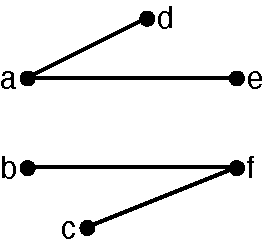
\includegraphics[width=0.9\linewidth]{figures/amb_value/0_amb_value.pdf}
        \caption{Straight-line graph}
        \label{fig:amb_value_0}
    \end{subfigure}
    \begin{subfigure}{0.3\linewidth}
        \centering
        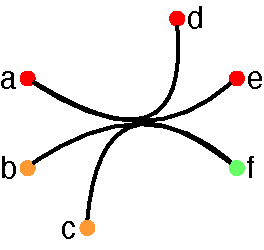
\includegraphics[width=0.9\linewidth]{figures/amb_value/1_amb_value.pdf}
        \caption{Bundled graph}
        \label{fig:amb_value_1}
    \end{subfigure}
  \caption{\subref{fig:amb_value_1} is a possible bundle of \subref{fig:amb_value_0}. In \subref{fig:amb_value_1}, all red nodes are false neighbors $N_{\Gamma}^f$ for the b node, and all yellow nodes are false neighbors $N_{\Gamma}^f$ for f. \cite{Straub2022}}
  \label{fig:ambiguity_2}
\end{figure}

To compare those three algorithms, we utilize the three quality metrics provided by Wallinger et al. \cite{wallinger_edge-path_2022} and modify them according to our needs. 
The ink reduction $ink(I)$ reveals how many edges were bundled and how much the bundling reduced the clutter by counting the non-white pixels in a plot. $I_B$ is the bundled plot and $I_O$ the original plot.

\begin{equation}
    ink(I)=\frac{\sum_{i=1}^m \sum_{j=1}^n I_B(i,j)}{\sum_{i=1}^m \sum_{j=1}^n I_O(i,j)}
\end{equation}

The bundling reduced clutter inside the graph if the number of non-white pixels shrank.
The next metric, $dist(\Gamma)$, tells if the bundled edges make a long detour or remain close to the Euclidean distance. Suppose they had a long detour that would make adjacencies harder to read. 

\begin{equation}
    dist(\Gamma)= \sum_{(u,v)\in E} \frac{d_{\Gamma}(u,v)}{||u-v||}
\end{equation}

The distortion value is calculated by dividing the length of the sum of the edges of the bundled graph by that of the original.
The ambiguity metric $amb(\Gamma)$ reveals the perceivable false connections within the bundled graph.

\begin{equation}
    amb(\Gamma)=\frac{\sum_{v \in V} \sum_{e=(v,w)\in E} |N_{\Gamma}^f(v,e)|}{\sum_{v \in V} \sum_{e=(v,w)\in E} |N_{\Gamma}(v,e)|}
\end{equation}

To calculate this, we divide all false neighbors by all possible neighbors. $N_{\Gamma}$ is the number of reachable neighbors from a node $x$ with edge $e$. $N_{\Gamma}^f$ are all false neighbours. \autoref{fig:ambiguity_2} is an example of the relationship between true and false neighbors.
A connection is ambiguous if two edges intersect with a slight angle or the distance between them is too small to distinguish them.
%%%%%%%%%%%%%%%%%%%%%%%%%%%%%%%%%%%%%%%%%%%%%%%%%%%%%%%%%%%%%%%%%%%%%%%%
% ************************************************************************
\begin{table*}[tb]
  \centering
  \setlength\tabcolsep{5pt} % adjust white space inside table
  \caption{
    \label{tab:quality}
    The table displays the quality metrics scores for our four synthetic data graphs. The bundled drawings for the \textbf{default} graph are displayed here \autoref{fig:default_bezier_steiner}, for the \textbf{10x10} graph here \autoref{fig:10x10_figure}, for the \textbf{15x15} graph here \autoref{fig:15x15_figure} and the \textbf{25x25} graph here \autoref{fig:25x25_figure}.
  }  
  \begin{tabular}{p{0.045\linewidth} || p{0.045\linewidth} p{0.045\linewidth} p{0.055\linewidth} | p{0.045\linewidth} p{0.045\linewidth} p{0.055\linewidth} | p{0.045\linewidth} p{0.045\linewidth} p{0.055\linewidth} | p{0.045\linewidth} p{0.045\linewidth} p{0.055\linewidth}}
    \toprule
     & \multicolumn{3}{c|}{\bfseries default} & \multicolumn{3}{c|}{\bfseries 10x10\_10n\_30e} & \multicolumn{3}{c|}{\bfseries 15x15\_10n\_40e} & \multicolumn{3}{c}{\bfseries 25x25\_10n\_30e}\\
     & $ink$ & $dist$ & $amb$ & $ink$ & $dist$ & $amb$ & $ink$ & $dist$ & $amb$ & $ink$ & $dist$ & $amb$ \\
    \midrule
    Org & 1.000 & 1.000 & 0.000 & 1.000 & 1.000 & 0.035 & 1.000 & 1.00 & 0.037 & 1.00 & 1.00 & 0.100 \\
    WR & 0.686 & \textbf{0.985} & \textbf{0.000} & 0.677 & \textbf{1.055} & 0.070 & 0.700 & \textbf{1.017} & \textbf{0.062} & \textbf{0.643} & \textbf{1.001} & \textbf{0.033} \\
    EPB & 1.553 & 1.321 & \textbf{0.000} & 1.368 & 1.169 & \textbf{0.053} & 1.167 & 1.179 & 0.075 & 1.513 & 1.177 & 0.100 \\
    PSB & \textbf{0.685} & 0.955 & \textbf{0.000} & \textbf{0.613} & 1.060 & 0.122 & \textbf{0.562} & 1.126 & 0.075 & 0.728 & 1.191 & 0.133 \\
    \bottomrule
  \end{tabular}
\end{table*}
% ************************************************************************

\begin{figure}[H]
    \begin{subfigure}{0.5\linewidth}
        \centering
        \includegraphics[width=\linewidth]{figures/10x10/original_10x10_10n_30e.png}
        \caption{Straight-line graph}
        \label{fig:original_10x10}
    \end{subfigure}
    \begin{subfigure}{0.5\linewidth}
        \centering
        \includegraphics[width=\linewidth]{figures/10x10/wr_10x10_10n_30e.png}
        \caption{Winding Roads}
        \label{fig:wr_10x10}
    \end{subfigure}
    \begin{subfigure}{0.5\linewidth}
        \centering
        \includegraphics[width=\linewidth]{figures/10x10/epb_10x10_10n_30e.png}
        \caption{Edge-Path bundling}
        \label{fig:epb_10x10}
    \end{subfigure}
    \begin{subfigure}{0.5\linewidth}
        \centering
        \includegraphics[width=\linewidth]{figures/10x10/10x10_10n_30e_12-1000.png}
        \caption{Physarium Steiner bundling}
        \label{fig:10x10}
    \end{subfigure}
  \caption{These are example solutions for a 10x10 grid graph. The original straight-line graph is presented in \subref{fig:original_10x10}. With these plots, the strike bundling of our method in \subref{fig:10x10} can be seen.
  As all three algorithms use different techniques to plot the graph, slight visual variations may be noticeable.}
  \label{fig:10x10_figure}
\end{figure}

\begin{figure}[H]
    \begin{subfigure}{0.5\linewidth}
        \centering
        \includegraphics[width=\linewidth]{figures/15x15/original_15x15_10n_40e.png}
        \caption{Straight-line graph}
        \label{fig:original_15x15}
    \end{subfigure}
    \begin{subfigure}{0.5\linewidth}
        \centering
        \includegraphics[width=\linewidth]{figures/15x15/wr_15x15_10n_40e.png}
        \caption{Winding Roads}
        \label{fig:wr_15x15}
    \end{subfigure}
    \begin{subfigure}{0.5\linewidth}
        \centering
        \includegraphics[width=\linewidth]{figures/15x15/epb_15x15_10n_40e.png}
        \caption{Edge-Path bundling}
        \label{fig:epb_15x15}
    \end{subfigure}
    \begin{subfigure}{0.5\linewidth}
        \centering
        \includegraphics[width=\linewidth]{figures/15x15/15x15_10n_40e_12-1000.png}
        \caption{Physarium Steiner bundling}
        \label{fig:15x15}
    \end{subfigure}
  \caption{These are example solutions for a 15x15 grid graph. The original straight-line graph is presented in \subref{fig:original_15x15}. Interestingly to us is that \subref{fig:epb_15x15} and \subref{fig:15x15} look similar in regards to their ink reduction, but their metrics in \autoref{tab:quality} do not confirm this observation. This is the only plot out of the three examples where the Physarium Steiner bundling looks similar to one of the other approaches in this chase Edge-Path bundling.
  As all three algorithms use different techniques to plot the graph, slight visual variations may be noticeable.}
  \label{fig:15x15_figure}
\end{figure}

\begin{figure}[H]
    \begin{subfigure}{0.5\linewidth}
        \centering
        \includegraphics[width=\linewidth]{figures/25x25/original_25x25_10n_30e.png}
        \caption{Straight-line graph}
        \label{fig:original_25x25}
    \end{subfigure}
    \begin{subfigure}{0.5\linewidth}
        \centering
        \includegraphics[width=\linewidth]{figures/25x25/wr_25x25_10n_30e_graph.png}
        \caption{Winding Roads}
        \label{fig:wr_25x25}
    \end{subfigure}
    \begin{subfigure}{0.5\linewidth}
        \centering
        \includegraphics[width=\linewidth]{figures/25x25/epb_25x25_10n_30e_graph.png}
        \caption{Edge-Path bundling}
        \label{fig:epb_25x25}
    \end{subfigure}
    \begin{subfigure}{0.5\linewidth}
        \centering
        \includegraphics[width=\linewidth]{figures/25x25/25x25_10n_30e_12-1000.png}
        \caption{Physarium Steiner bundling}
        \label{fig:25x25}
    \end{subfigure}
  \caption{These are example solutions for a 25x25 grid graph. The original straight-line graph is presented in \subref{fig:original_25x25}. With these plots, it is easy to spot the striker bundling approach of \subref{fig:25x25}. All long edges that remain relatively straight and original are merged into the main bundle in the middle.
  As all three algorithms use different techniques to plot the graph, slight visual variations may be noticeable.}
  \label{fig:25x25_figure}
\end{figure}

\section{Comparison}
\label{sec:comparison}

As mentioned in \autoref{sec:testing}, our algorithm is too slow to solve real-world graphs, and we, therefore, rely on synthetic data we generated. The default dataset has six nodes and was the graph we tested new features throughout the testing phase, as it is fast to calculate, and the resulting Steiner tree is known. It is also the only graph that is not randomly generated. The others get increasingly complex and grow in size. The increasing complexity was done to test the limits and see the behavior of the calculation \autoref{tab:quality}. 

\subsection{Ink Reduction}
\label{sec:ink_reduction}
Logically the ink reduction of the straight-line graph is one. Edge path bundling performs the worst in this category as it uses the shortest edges of the existing path network and a B\'{e}zier curve to visualize the longest paths. Winding Roads and our approach have a much higher degree of bundling, as both use an underlying structure to bundle. That the Physarium Steiner bundling comes out on top is to be expected, as it has a smaller frame to work with. The scores also fit the appearance of \autoref{fig:10x10}, \autoref{fig:15x15} and \autoref{fig:25x25}.

\subsection{Distortion}
\label{sec:distortion}
The distortion on a straight-line graph is, by definition, one. With this metric, the results are much closer, and Winding roads has the least distorted bundling. We observe that the distortion value of our approach is linked to the graph size; the larger the graph, the higher the distortion value. The high distortion value means that the greater the graph gets, the longer the detours of the paths must be, compared to their original counterparts. The longer detours exist because all paths must use the Steiner tree for their routing and if the graph increases in size, the detour through the Steiner tree becomes more significant than the direct path.

\subsection{Ambiguity}
\label{sec:ambiguity}
As even straight-line graphs can have ambiguities, it is to be expected that a low ambiguity value is present. Both Winding Roads and Edge Path bundling have only a slightly larger ambiguity value than the straight-line graph. These are caused by edge crossings which a shallow crossing angle. On the other hand, our approach consistently has the most ambiguities as the proximity of paths causes them. This results in a compact graph whose side effect is that it is more challenging to follow paths.
%%%%%%%%%%%%%%%%%%%%%%%%%%%%%%%%%%%%%%%%%%%%%%%%%%%%%%%%%%%%%%%%%%%%%%%%


  %!TEX root = ../Thesis.tex

%%%%%%%%%%%%%%%%%%%%%%%%%%%%%%%%%%%%%%%%%%%%%%%%%%%%%%%%%%%%%%%%%%%%%%%%
\chapter{Conclusion}
\label{sec:conclusion}

This work introduced a novel edge bundling technique based on a Physarium approximation of a Steiner tree. This Steiner tree is then used as a routing structure for graph paths. We evaluated and compared our algorithm using the quality metrics: ink reduction, distortion, and ambiguity. These metrics are computed on graph drawings of synthetic data we generated for testing pursues. The resulting illustrations consist of dense graphs that reduce node-edge overlaps, make reading easier, and make it more straightforward to spot areas of interest. Our algorithm has a worst-case complexity of $O\left(T_0 \cdot \left(n \cdot e + T_i\left(n^3\right)\right)\right)$ which is enough for small-scale synthetic graphs, but not enough to be used with real-world data, mainly because graph bundling becomes necessary if the graph data it too large to comprehend. 

The metrics comparison showed us that our approach has a reasonable degree of bundling and outperforms the other two techniques. This, however, comes at the cost of distortion and ambiguity. Nevertheless, the excellent ink reduction value is a promising sign that with a better approximation algorithm, our approach could be used to declutter graphs and isolate regions of interest. 

For us, future work could lead in two directions. The first would be to improve performance by using a GPU-based implementation to solve the matrices or abandoning the Physarium approximation and instead employ GeoSteiner \cite{winter_euclidean_1997}, or even better SCIP-Jack \cite{RehfeldtKoch2023} for a fast Steiner tree approximation. The other direction would be to utilize the Physarium-inspired approach to a Euclidean Steiner tree by Hsu \cite{hsu_physarum-inspired_2022}. With this, it should be possible to bundle real-world graph data.

To conclude: Our approach suffers from significant drawbacks caused by the slow approximation calculation, which hindered us from testing real-world graph data and, in turn, evaluating the usefulness of our method. Unfortunately, we discovered too late that our optimizations could not improve the approximation enough to become functional. 
Nevertheless, we still think it is a promising approach that could become feasible by utilizing the above-mentioned future work. 
%%%%%%%%%%%%%%%%%%%%%%%%%%%%%%%%%%%%%%%%%%%%%%%%%%%%%%%%%%%%%%%%%%%%%%%%  

% This ensures that the subsequent sections are being included as root
% items in the bookmark structure of your PDF reader.
\bookmarksetup{startatroot} 
\backmatter
  
  \printbibliography
  
\end{document}